\chapter{Preparation}


\section{Design of an awesome resonator}
To filter a special wavelength using a ring resonator the design of the resonator needs to be adjusted to the wavelength.
\begin{figure}[h]%
\centering
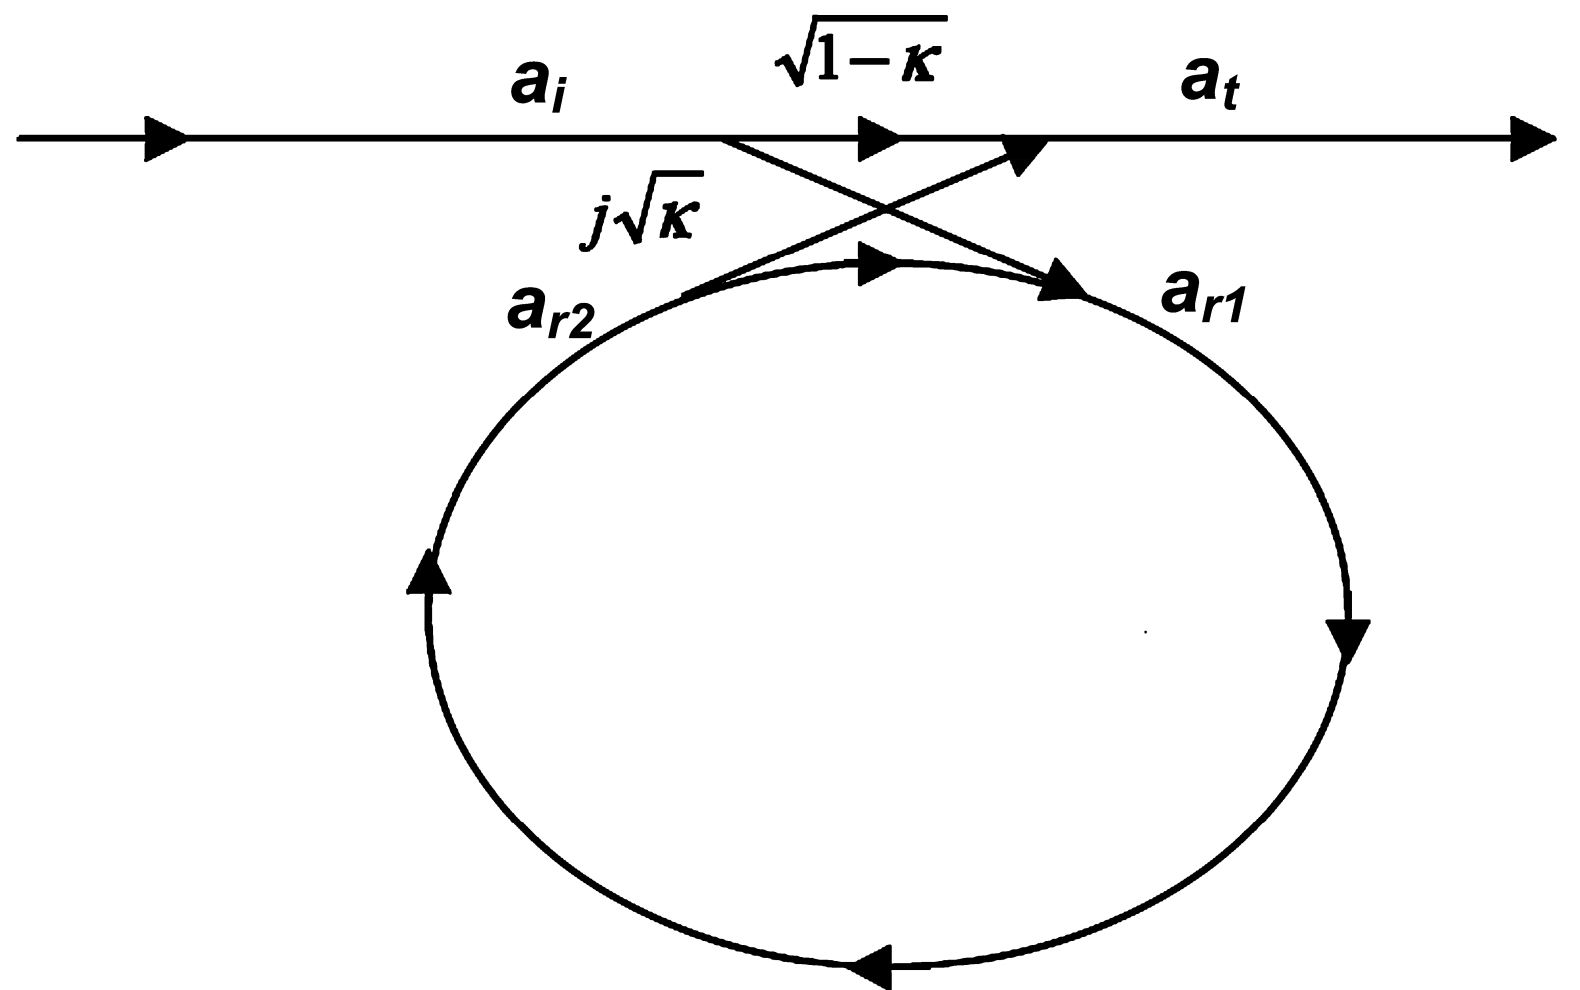
\includegraphics[width=.5\columnwidth]{Grafiken/Resonator.png}%
\caption{Schematic of a ring resonator.}%
\label{fig:p1_ring}%
\end{figure} 
Figure \ref{fig:p1_ring}\footnote[1]{Jingshi Li, Materials for the preparation of Experiment 6} shows a schematic picture of a parallel ring resonator. It consists of a coupling zone between the ring resonator and the waveguide which can be modelled as directional coupler\footnotemark[1].

The transmission of the ring follows the relation:

\begin{equation}
a\i{r2}=a_{\mathrm{r1}}\cdot e^{-a/2\cdot L}\cdot e^{-j\beta L}
\label{eq:}
\end{equation}
That means the ring is in resonance
\begin{equation}
\beta L = m\cdot2\pi,\qquad m \in \mathbf{N}
\label{eq:}
\end{equation}
wiht $\beta = n_{\mathrm{eff}} \frac{2\pi f}{c} = n_{\mathrm{eff}} \frac{2\pi}{\lambda_0}$.

Using the transmission of the ring and the matrix of the directional coupler a term for the transmittet power can be derived\footnotemark[1]:
\begin{equation}
T(\beta L) = \frac{|a_t|^2}{|a_i|^2}= \frac{(1-e^{-a\cdot L})(1-(1-\kappa))}{(1-e^{-a/2\cdot L}\sqrt{1-\kappa})^2+4e^{-a/2\cdot L}\sqrt{1-\kappa}\cdot\mathrm{sin}^2(\beta L / 2)}}
\label{eq:}
\end{equation}
As described above the ring is in resonance for $\beta L = m\cdot2\pi$ and the transmission becomes minimum. 
In this case
\begin{equation}
T_{\mathrm{min}}=\frac{(e^{-a/2\cdot L} - \sqrt{1-\kappa})^2}{(1 - e^{-a/2\cdot L}\sqrt{1-\kappa})^2}
\label{eq:}
\end{equation}

When $e^{-a/2\cdot L} = \sqrt{1-\kappa}$ the transmission is zero. This case is calld $critical~coupling$ and can be achieved for $a = - \frac{1}{L}\mathrm{ln}(1-\kappa)$.

To design ring resonator filter to block certain wavelength there are different approaches.
At first the filter could be consist different in series connected parallel ring resonators. Each resonator would filter characteristic frequencies.
For the given wavelenght $\lambda_1 = 1550$~nm and $\lambda_2 = 1551$~nm two other approaches are conceivable.

Firstly one resonator could be used with a resonance frequency between $\lambda_1$ and $\lambda_2$. If the width of the resonance line is broader than than the difference between $\lambda_1$ and $\lambda_2$ both wavelengths get filtered.

Secondly the design of the waveguide used for the ring resonator (material, dimensions) could be chosen, that the effective indices for the two waveguides are just so that 

\begin{equation}
\frac{2\pi n_{\mathrm{eff,1}}}{\lambda_1} = \frac{2\pi n_{\mathrm{eff,2}}}{\lambda_2}
\label{eq:}
\end{equation}
is true.


\section{Measuring the Resonator Parameters}

\begin{figure}[h]%
\centering
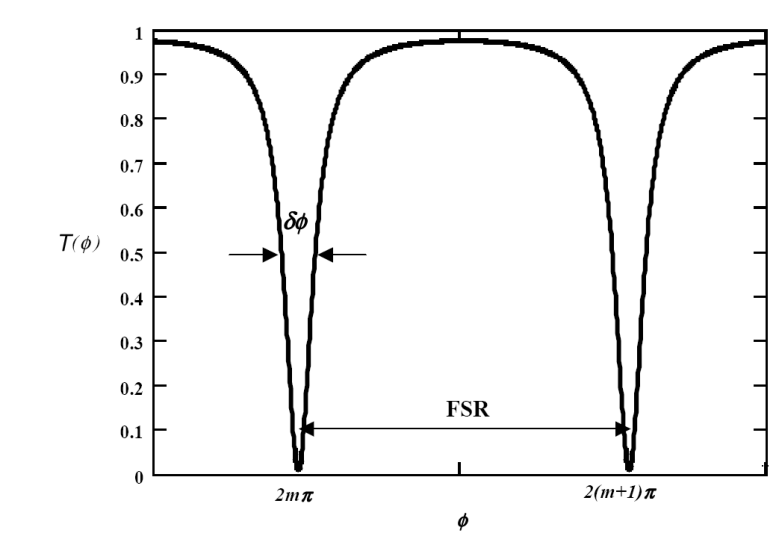
\includegraphics[width=.5\columnwidth]{Grafiken/S21.pdf}%
\caption{Example Transmission Coefficient of a Resonator}%
\label{fig:S21}%
\end{figure}
\todo{Bild evtl auf f anpassen}

To caracterize a resonator its power transmission in dependency of the frequency can easily be measured. By that measurement, the whidth of the resonance lines at full width half maximum (FWHM) $\delta f$ and the free spectral range $\Delta f$ can determined. (cf. figure \ref{fig:S21}). The quotient $F= \Delta f/\delta f$ is called Finesse. For the case of critical coupling $F$ is given as:
\begin{equation}
 F = \frac{\Delta f}{\delta f} = \frac{\pi\sqrt{1-\kappa}}{\kappa}=\frac{\pi\exp\left(-\alpha/2L\right)}{1-\exp\left(-\alpha/L\right)}
\end{equation}
This can be rearranged to:
\begin{equation}
 \kappa = 0.5 \pm \sqrt{0.25+F^2/\pi^2}
\end{equation}
and
\begin{equation}
\alpha = -\frac{\ln F}{L(\ln F+2\ln\pi)} 
\end{equation}
respectively.

\section{Over-Critical and Under-Critical coupling}
